\documentclass{article}
\usepackage{graphicx}
\usepackage{alltt}
\usepackage{amsmath}
\usepackage{amsfonts}
\usepackage{bigstrut}
\usepackage{enumerate}
\usepackage{fancyhdr}
\usepackage[top=.75in, bottom=.95in, left=.75in, right=.75in]{geometry}
\usepackage{float}
\usepackage{lastpage}
\usepackage{tikz}
\usepackage[latin1]{inputenc}
\usepackage{color}
\usepackage{array}
\usepackage{longtable}
\usepackage{calc}
\usepackage{multirow}
\usepackage{hhline}
\usepackage{ifthen}
\usepackage{listings}
\usepackage{circuitikz}
\usepackage{caption}
\definecolor{mygreen}{rgb}{0,0.6,0}
\definecolor{mygray}{rgb}{0.5,0.5,0.5}
\definecolor{mymauve}{rgb}{0.58,0,0.82}
\lstset{ %
  backgroundcolor=\color{white},   % choose the background color; you must add \usepackage{color} or \usepackage{xcolor}; should come as last argument
  basicstyle=\normalsize,        % the size of the fonts that are used for the code
  breakatwhitespace=false,         % sets if automatic breaks should only happen at whitespace
  breaklines=true,                 % sets automatic line breaking
  captionpos=b,                    % sets the caption-position to bottom
  commentstyle=\color{mygreen},    % comment style
  deletekeywords={...},            % if you want to delete keywords from the given language
  escapeinside={\%*}{*)},          % if you want to add LaTeX within your code
  extendedchars=true,              % lets you use non-ASCII characters; for 8-bits encodings only, does not work with UTF-8
  frame=single,	                   % adds a frame around the code
  keepspaces=true,                 % keeps spaces in text, useful for keeping indentation of code (possibly needs columns=flexible)
  keywordstyle=\color{blue},       % keyword style
  language=python,                  % the language of the code
  morekeywords={*,...},            % if you want to add more keywords to the set
  numbers=left,                    % where to put the line-numbers; possible values are (none, left, right)
  numbersep=5pt,                   % how far the line-numbers are from the code
  numberstyle=\tiny\color{mygray}, % the style that is used for the line-numbers
  rulecolor=\color{black},         % if not set, the frame-color may be changed on line-breaks within not-black text (e.g. comments (green here))
  showspaces=false,                % show spaces everywhere adding particular underscores; it overrides 'showstringspaces'
  showstringspaces=false,          % underline spaces within strings only
  showtabs=false,                  % show tabs within strings adding particular underscores
  stepnumber=2,                    % the step between two line-numbers. If it's 1, each line will be numbered
  stringstyle=\color{mymauve},     % string literal style
  tabsize=2,	                   % sets default tabsize to 2 spaces
  title=\lstname                   % show the filename of files included with \lstinputlisting; also try caption instead of title
}
\floatstyle{boxed}
\floatstyle{plain}
\restylefloat{figure}
\pagestyle{fancy}
\fancyhead{}
\fancyfoot{}
\setlength{\headheight}{59.0pt}
\def\inputGnumericTable{}
\fancyhead[CO]{\textbf{Air Force Institute of Technology\\Department of Electrical and Computer Engineering\\
 Computer Communication Networks (CSCE-654) Project \#1\newline \newline Name: Micah Hayden}}
\lhead{\today}
\rhead{Page \thepage{} of \pageref{LastPage} }
\newlength\tindent
\setlength{\tindent}{\parindent}
\setlength{\parindent}{0pt}
\renewcommand{\indent}{\hspace*{\tindent}}
\begin{document}

%\begin{abstract}
%This is my abstract.
%\end{abstract}

\section*{Omnet Simulation Setup:}
I utilized the provided FIFO queue sample project as my starting point.
I needed to make the following changes to ensure I had a working simulation for the task:

\begin{enumerate}
	\item \textbf{FifoNet.ned}  

This file defines the "FifoNet" setup.  I created three identical queues consisting of a source node, a FIFO server, and a sink node, in which all traffic flows through the three nodes; this setup is shown in Figure \#\ref{diagram}.  

\begin{figure}[h!]
	\begin{center}
	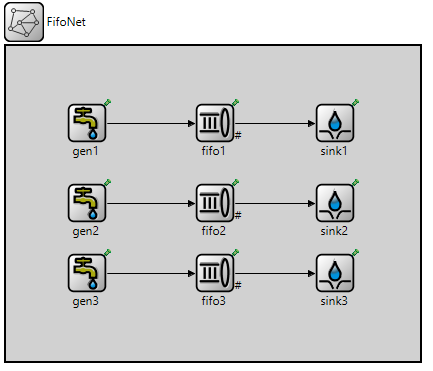
\includegraphics[scale=1.0]{Images/FifoNet.PNG}
	\vspace{-.25cm}
	\caption{Diagram showing the three queue setup.}
	\label{diagram}
	\end{center}
\end{figure}

When a packet arrives at the sink, it generates a packet delay data point as defined in Eq. \#\ref{delay}
\begin{equation}
	\label{delay}
	Packet \, Delay = time_{arrival} - time_{created}
\end{equation}

	\item \textbf{omnetpp.ini}
	
The modifications to this file specified each queue's individual parameters.  Each queue had a \textbf{service time} of $t_s = 0.75 \, seconds$.
I differentiated the arrival rates of each queue by specifying the interarrival time from each generator/source.
These times are shown below:

\begin{table}[h!]
\centering
\begin{tabular}{|c|c|} \hline
\textbf{Queue \#:} & \textbf{ Interarrival Time (seconds)} \\ \hline
1 & 1.0 \\ \hline
2 & 0.50 \\ \hline
3 & 0.25 \\ \hline
\end{tabular}
\caption{Interarrival Times}
\label{InterarrivalTimes}
\end{table}

The final change was to set the \textbf{sim-time-limit} to one hour.
\end{enumerate}

\newpage
\section*{Results \& Analysis:}
\subsection*{Utilization:}
Given the interarrival times and service times of each queue, I calculated values for $\lambda, \, \mu, \, \mathrm{and} \, \rho$ for each queue using the below relationships:

\begin{align*}
\lambda = \frac{1}{Interarrival \, Time} \hspace{1 cm} \mu = \frac{1}{Service \, Time} \hspace{1cm} \rho = \frac{\lambda}{\mu}
\end{align*}

Note, each queue has a service time of 0.75 seconds, and the interarrival times stated in Table \#\ref{InterarrivalTimes}

\begin{table}[h!]
\centering
\begin{tabular}{|c|c|c|c|} \hline
\textbf{Queue \#:} & $\mathbf{\lambda}$ & $\mathbf{\mu}$ & $\mathbf{\rho}$ \\ \hline
1 & 1.00 & $1.\bar{33}$ & 0.75  \\ \hline
2 & 2.00 & $1.\bar{33}$ & 1.50 \\ \hline
3 & 4.00 & $1.\bar{33}$ & 3.00\\ \hline
\end{tabular}
\caption{Utilization}
\label{Utilization}
\end{table}

Given the values of utilization ($\rho$) shown in Table \#\ref{Utilization} above, I would expect Queue \#1 to have a negligible delay.  However, Queues \#2 and \#3 will have a queue length which will grow to infinity because $\rho > 1$. 
This makes sense given the meaning of each variable:  for Queue \#1 - packets arrive slower than they are serviced, for the other two queues - packets arrive faster than they can be serviced.

\subsection*{System Delay}
Figure \#\ref{DelayPlot} shows the system delay of each queue, where sinks \#1-3 correspond to Queues \#1-3.

\begin{figure}[h!]
	\begin{center}
	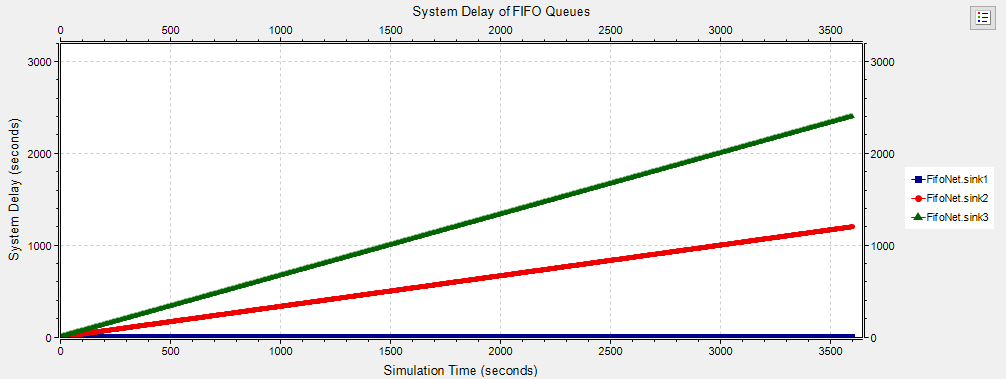
\includegraphics[scale=0.65]{Images/DelayPlot.PNG}
	\vspace{-.25cm}
	\caption{System Delay of Queues \#1-3}
	\label{DelayPlot}
	\end{center}
\end{figure}

Packets in Queue \#1 experienced $delay = service \, time$.  However, for Queue \#2 and Queue \#3, their system delays increased rapidly as the queue length increased.  Despite the differences in arrival rates between Queue \#2 and \#3, they both serviced 4800 packets, which is the maximum possible in one hour with a service time = $0.75 \, seconds$.
This occurs because both of those queues had a utilization $> 1$.  
Queue \#1 serviced each packet which arrived, servicing a total of 3600 packets.

\newpage
\subsection*{Queue Length \& Queue Time}
Tables \#3 and \#4 below show the raw data for the queue length and queue time for each queue.\footnote{The count seems increased by 1, but is caused by the packets arriving at the end of the simulation, that had not been serviced.}
\vspace{.25cm}

\begin{minipage}{0.5\textwidth}
	\centering
	\begin{tabular}{|c|c|c|c|} \hline
		\textbf{Queue \#} & \textbf{Count} & \textbf{Mean} & \textbf{Std. Dev} \\ \hline
		1 & 1 & 0.0 & 0.00 \\ \hline
		2 & 12001 & 1200.0 & 692.91 \\ \hline
		3 & 19201 & 4800.3 & 2771.50 \\ \hline
	\end{tabular}
	\captionof{table}{Queue Length}
	\label{qlen}
\end{minipage}  
\begin{minipage}{0.5\textwidth}
	\centering
	\begin{tabular}{|c|c|c|c|} \hline
		\textbf{Queue \#} & \textbf{Count} & \textbf{Mean} & \textbf{Std. Dev} \\ \hline
		1 & 3601 & 0.0 & 0.00 \\ \hline
		2 & 4801 & 600.0 & 346.52 \\ \hline
		3 & 4801 & 1200.0 & 693.04 \\ \hline
	\end{tabular}
	\captionof{table}{Queue Time}
	\label{qTime}
\end{minipage}
\vspace{.25cm}

The data shown above is indicative of the system delays experienced by each packet.
When the server can keep up with/stay ahead of the queue, arriving packets have no queuing delay:  there is no queue!
However, once the queue forms, if the arrival rate remains faster than the service rate, the queue simply continues to grow, causing increasing system delays for each packet.

\newpage

\section*{Appendix A:  Edited Files}

\begin{figure}[H]
\label{FifoNet}
\begin{lstlisting}
// FifoNet.ned:
network FifoNet
{
    submodules:
        gen1: Source {
            parameters:
                @display("p=81,77");
        }
        gen2: Source {
            parameters:
                @display("p=81,157");
        }
        gen3: Source {
            parameters:
                @display("p=81,227");
        }
        fifo1: Fifo {
            parameters:
                @display("p=209,77");
        }
        fifo2: Fifo {
            parameters:
                @display("p=209,157");
        }
        fifo3: Fifo {
            parameters:
                @display("p=209,227");
        }
        sink1: Sink {
            parameters:
                @display("p=329,77");
        }
        sink2: Sink {
            parameters:
                @display("p=329,157");
        }
        sink3: Sink {
            parameters:
                @display("p=329,227");
        }
    connections:
        gen1.out --> fifo1.in;
        fifo1.out --> sink1.in;

        gen2.out --> fifo2.in;
        fifo2.out --> sink2.in;

        gen3.out --> fifo3.in;
        fifo3.out --> sink3.in;
}
\end{lstlisting}
\vspace{-1cm}
\caption*{Defining the network in FifoNet.ned}
\end{figure}

\begin{figure}[H]
\label{Omnet_ini}
\begin{lstlisting}
// omnetpp.ini
[General]
description = "3 Seperate Arrival times, same service times"
network = FifoNet
sim-time-limit = 1h
cpu-time-limit = 300s
#debug-on-errors = true
#record-eventlog = true
**.gen1.sendIaTime = 1s
**.fifo1.serviceTime = 0.75s

**.gen2.sendIaTime = 0.50s
**.fifo2.serviceTime = 0.75s

**.gen3.sendIaTime = 0.25s
**.fifo3.serviceTime = 0.75s
\end{lstlisting}
\vspace{-1cm}
\caption*{Omnetpp.ini edited to run the three queues with separate parameters}
\end{figure}

\end{document}